\section{Experimentation}
\par We implement the feature extraction framework and the model architectures in PyTorch. We show that our model achieves competitive results compared to current state-of-the-art models with fewer training epochs and even fewer attention tokens. We utilize multimodal features from ViViT and AST encoders, pretrained using our adapted Temporally Sensitive Pretraining framework. The ActivityNet dataset is used, which is the largest available dataset for the task of Dense Video Captioning.

\subsection{Feature Preprocessing Details}
\par We standardize all videos in the ActivityNet Captions dataset to 30 frames per second (30fps) and audio sampling rate of 44100Hz. For feature extraction as well as temporally sensitive pretraining, we use 16 frames per clip and sample 5 clips per segment in the dataset. We use 128 Mel bins and a target length of 64 for audio input. We start training the ViViT and AST encoders from Kinetics pretrained weights and Audioset pretrained weights respectively. ViViT uses a spatial patch size of $16 \times 16$, and a temporal patch size of 2. The number of encoder layers of ViViT and AST is kept 12. We train these encoders with a batch size of 8 and a stochastic gradient descent optimizer with momentum and weight decay.

\subsection {Training Details}
\par We train our model across 4 DGX-A100 GPUs for 70 epochs with an NCCL backend and a batch size of 16 for 60 hours. We use the AdamW optimizer with a learning rate of $10^{-4}$. We also use gradient clipping with a maximum threshold of $0.1$ to avoid exploding gradients. We set the model's embedding dimension to 512, with 6 layers and 8 attention heads for the transformer encoder, decoder and captioning module. Thus, our model has 75M parameters, excluding the feature extraction encoders. 
\par The smoothing rate $\alpha$ (for caption loss) is set to $0.5$. We initialize all transformer weights using the Xavier initialized distribution \cite{xavier}. We also use $sine$ positional embeddings, adapted for videos by accounting for their duration. We set the number of \textit{event queries} to 20 and the maximum event counter length to 10.
\par For the deformable attention head, we use 4 feature levels with 4 sampling sampling points per attention head and a 2048-dimensional FFN. We set $\rho$ to 0.5 (utilize only 50\% tokens) and dropout as 0.1.
\par For calculating the Hungarian loss, we perform a linear combination across all individual losses. Their corresponding coefficients are $\alpha_{l1}=5, \alpha_{giou}=2, \alpha_{event}=2, \alpha_m=3, \alpha_{cap}=1$.

\subsection {Evaluation Metrics}
\par We use 2 different metric sets to evaluate different aspects of our model.
\begin{itemize}
	\item For evaluating the event boundaries, we use Precision and Recall across IoU thresholds at $\left \{0.3, 0.5, 0.7, 0.9 \right\}$ along with an average across all the thresholds. We also calculate the corresponding average F1 score.
	\item For evaluating the captions, we calculate the BLEU \cite{bleu} scores across 4 thresholds at $\left \{1, 2, 3, 4\right\}$, METEOR \cite{meteor} and CIDEr \cite{cider}, based on the official ActivityNet challenge guidelines. We also calculate the ROUGE-L \cite{rouge} scores for the captions.
\end{itemize}

\section{Results}

Our model achieves competitive results for both, the event localization and event captioning tasks across most metrics. The following tables show the results of the comparison for captioning and event localization against popular previous works, each with different model architectures and training paradigms.
% Please add the following required packages to your document preamble:
% \usepackage{multirow}
\begin{table}[h] \label{table:capeval}
	\centering
	\begin{tabular}{|c|cclllcc|}
		\hline
		\multirow{2}{*}{\textbf{Paper}}        & \multicolumn{7}{c|}{\textbf{Learnt Proposals}}                                                                                                                                                                                                                        \\ \cline{2-8} 
		& \multicolumn{1}{c|}{M}             & \multicolumn{1}{c|}{C}              & \multicolumn{1}{c|}{R}               & \multicolumn{1}{l|}{B@1}             & \multicolumn{1}{l|}{B@2}           & \multicolumn{1}{c|}{B@3}           & B@4                                \\ \hline
		{Krishna \textit{et al} \cite{krishna2017densecaptioning} DCE}                                 & \multicolumn{1}{c|}{5.69}          & \multicolumn{1}{c|}{12.43}          & \multicolumn{1}{l|}{}                & \multicolumn{1}{l|}{10.81}           & \multicolumn{1}{l|}{4.57}          & \multicolumn{1}{c|}{1.90}          & 0.71                               \\ \hline
		{Zhou \textit{et al} \cite{zhou2018end} Masked Transformer}                & \multicolumn{1}{c|}{4.98}          & \multicolumn{1}{c|}{9.25}           & \multicolumn{1}{l|}{}                & \multicolumn{1}{l|}{9.96}            & \multicolumn{1}{l|}{4.81}          & \multicolumn{1}{c|}{2.42}          & 1.15                               \\ \hline
		{Wang \textit{et al} \cite{wang2018bidirectional} Bi-SST}                       & \multicolumn{1}{c|}{5.86}          & \multicolumn{1}{c|}{7.99}           & \multicolumn{1}{l|}{\textbf{19.29}}           & \multicolumn{1}{l|}{\textbf{19.37}}           & \multicolumn{1}{l|}{\textbf{8.84}}          & \multicolumn{1}{c|}{2.55}          & 1.31                               \\ \hline
		{Li \textit{et al} \cite{li2018jointly} Descriptivness Regr.}          & \multicolumn{1}{c|}{6.93}          & \multicolumn{1}{c|}{13.21}          & \multicolumn{1}{l|}{}                & \multicolumn{1}{l|}{12.22}           & \multicolumn{1}{l|}{5.72}          & \multicolumn{1}{c|}{2.27}          & 0.74                               \\ \hline
		{Mun \textit{et al} \cite{mun2019streamlined} Streamlined DVC}               & \multicolumn{1}{c|}{8.82}          & \multicolumn{1}{c|}{30.68}          & \multicolumn{1}{l|}{}                & \multicolumn{1}{l|}{17.92}           & \multicolumn{1}{l|}{7.99}          & \multicolumn{1}{c|}{2.94}          & 0.93                               \\ \hline
		Rahman \textit{et al} \cite{rahman2019watch} Watch, Listen, Tell       & \multicolumn{1}{c|}{4.93}          & \multicolumn{1}{c|}{13.79}          & \multicolumn{1}{l|}{10.39}           & \multicolumn{1}{l|}{10}              & \multicolumn{1}{l|}{4.2}           & \multicolumn{1}{c|}{1.85}          & 0.9                                \\ \hline
		Suin \textit{et al} \cite{suin2020efficient} Efficient framework for DVC & \multicolumn{1}{c|}{6.21}          & \multicolumn{1}{c|}{13.82}          & \multicolumn{1}{l|}{}                & \multicolumn{1}{l|}{}                & \multicolumn{1}{l|}{}              & \multicolumn{1}{c|}{2.87}          & 1.35                               \\ \hline
		Iashin \textit{et al} \cite{iashin2020multimodal} Multi-modal DVC            & \multicolumn{1}{c|}{7.31}          & \multicolumn{1}{l|}{}               & \multicolumn{1}{l|}{}                & \multicolumn{1}{l|}{}                & \multicolumn{1}{l|}{}              & \multicolumn{1}{c|}{2.6}           & 1.07                               \\ \hline
		Iashin \textit{et al} \cite{iashin2020better} BMT                       & \multicolumn{1}{c|}{8.44}          & \multicolumn{1}{l|}{}               & \multicolumn{1}{l|}{}                & \multicolumn{1}{l|}{}                & \multicolumn{1}{l|}{}              & \multicolumn{1}{c|}{\textbf{3.84}}          & 1.88                               \\ \hline
		Xiong \textit{et al} \cite{xiong2018forward} Move Forward and Tell      & \multicolumn{1}{c|}{7.08}          & \multicolumn{1}{l|}{}               & \multicolumn{1}{l|}{}                & \multicolumn{1}{l|}{}                & \multicolumn{1}{l|}{}              & \multicolumn{1}{c|}{2.84}          & 1.24                               \\ \hline
		{Wang \textit{et al} \cite{wang2020densecaptioning} SYSU}                        & \multicolumn{1}{c|}{\textbf{10.31}}         & \multicolumn{1}{l|}{}               & \multicolumn{1}{l|}{}                & \multicolumn{1}{l|}{}                & \multicolumn{1}{l|}{}              & \multicolumn{1}{c|}{}              &                                    \\ \hline
		Chadha \textit{et al} \cite{chadha2020iperceive} iPerceive                 & \multicolumn{1}{c|}{7.87}          & \multicolumn{1}{l|}{}               & \multicolumn{1}{l|}{}                & \multicolumn{1}{l|}{}                & \multicolumn{1}{l|}{}              & \multicolumn{1}{c|}{2.93}          & 1.29                               \\ \hline
		Song \textit{et al} \cite{songruc} RUC Sequential Events                 & \multicolumn{1}{c|}{8.82}          & \multicolumn{1}{l|}{30.68}               & \multicolumn{1}{l|}{}                & \multicolumn{1}{l|}{17.92}                & \multicolumn{1}{l|}{7.99}              & \multicolumn{1}{c|}{2.94}          & 0.93                               \\ \hline
		Deng \textit{et al} \cite{deng2021sketch} Sketch, Ground and Refine   & \multicolumn{1}{c|}{9.37}          & \multicolumn{1}{c|}{22.12}          & \multicolumn{1}{l|}{}                & \multicolumn{1}{l|}{14.05}           & \multicolumn{1}{l|}{}              & \multicolumn{1}{c|}{}              & 1.67                               \\ \hline
		Chen \textit{et al} \cite{chen2021towards} Towards Bridging EC-SL      & \multicolumn{1}{c|}{7.49}          & \multicolumn{1}{c|}{21.21}          & \multicolumn{1}{l|}{13.02}           & \multicolumn{1}{l|}{13.36}           & \multicolumn{1}{l|}{5.96}          & \multicolumn{1}{c|}{2.78}          & 1.33                               \\ \hline
		{Alwassel \textit{et al} \cite{alwassel2021tsp} TSP with BMT}            & \multicolumn{1}{c|}{8.75}          & \multicolumn{1}{l|}{}               & \multicolumn{1}{l|}{}                & \multicolumn{1}{l|}{}                & \multicolumn{1}{l|}{}              & \multicolumn{1}{c|}{4.16}          & \textbf{2.02}                               \\ \hline
		Wang \textit{et al} \cite{wang2021endtoend} Parallel decoding           & \multicolumn{1}{c|}{8.08}          & \multicolumn{1}{c|}{28.59}          & \multicolumn{1}{l|}{}                & \multicolumn{1}{l|}{}                & \multicolumn{1}{l|}{}              & \multicolumn{1}{c|}{}              & 1.96                               \\ \hline
		\textbf{Our model (video only)}                     & \multicolumn{1}{c|}{\textbf{6.42}} & \multicolumn{1}{l|}{\textbf{30.22}} & \multicolumn{1}{l|}{\textbf{13.58}} & \multicolumn{1}{l|}{\textbf{13.44}} & \multicolumn{1}{l|}{\textbf{4.12}} & \multicolumn{1}{l|}{\textbf{1.88}} & \multicolumn{1}{l|}{\textbf{0.44}} \\ \hline
		\textbf{Our model (video \& audio)}                     & \multicolumn{1}{c|}{\textbf{6.61}} & \multicolumn{1}{l|}{\textbf{31.38}} & \multicolumn{1}{l|}{\textbf{14.46}} & \multicolumn{1}{l|}{\textbf{15.36}} & \multicolumn{1}{l|}{\textbf{6.09}} & \multicolumn{1}{l|}{\textbf{2.28}} & \multicolumn{1}{l|}{\textbf{0.80}} \\ \hline
	\end{tabular}
	
	\centering
	\caption{Performance comparison of previous methods on the ActivityNet Captions dataset (*some videos unavailable)}  \label{tab: performance-comparison}
	
\end{table}

% Please add the following required packages to your document preamble:
% \usepackage{multirow}
\begin{table}[]
	\centering
	\begin{tabular}{|c|ccc|}
		\hline
		\multirow{2}{*}{\textbf{Paper}} & \multicolumn{3}{c|}{\textbf{Learnt Proposals}}                                             \\ \cline{2-4} 
		& \multicolumn{1}{c|}{Precision}      & \multicolumn{1}{c|}{Recall}         & F1             \\ \hline
		Zhou \textit{et al} \cite{zhou2017automatic} ProcNets                   & \multicolumn{1}{c|}{30.4}           & \multicolumn{1}{c|}{37.1}           & 33.42          \\ \hline
		Iashin \textit{et al} \cite{iashin2020better} BMT                             & \multicolumn{1}{c|}{48.23}          & \multicolumn{1}{c|}{\textbf{80.31}}          & 60.27          \\ \hline
		{Wang \textit{et al} \cite{wang2018bidirectional} Bi-SST}             & \multicolumn{1}{c|}{44.8}           & \multicolumn{1}{c|}{57.6}           & 50.40          \\ \hline
		Wang \textit{et al} \cite{wang2021endtoend} Parallel decoding                            & \multicolumn{1}{c|}{58.07}          & \multicolumn{1}{c|}{55.42}          & 56.71          \\ \hline
		{Mun \textit{et al} \cite{mun2019streamlined} Streamlined DVC}                 & \multicolumn{1}{c|}{57.57}          & \multicolumn{1}{c|}{55.58}          & 56.56          \\ \hline
		Song \textit{et al} \cite{songruc} RUC Sequential Events           & \multicolumn{1}{c|}{58.65}          & \multicolumn{1}{c|}{55.79}          & 57.18          \\ \hline
		\textbf{Our model (video)}              & \multicolumn{1}{c|}{\textbf{62.14}} & \multicolumn{1}{c|}{\textbf{61.25}} & \textbf{61.69} \\ \hline
		\textbf{Our model (video \& audio)}              & \multicolumn{1}{c|}{\textbf{66.25}} & \multicolumn{1}{c|}{\textbf{65.92}} & \textbf{66.08} \\ \hline
	\end{tabular}

	\centering
	\caption{Precision-Recall comparison of previous methods on the ActivityNet Captions dataset (*Some videos unavailable)}  \label{tab: precision-recall-comparison}
\end{table}


\begin{figure}[h]	
    \begin{subfigure}[b]{\linewidth}
	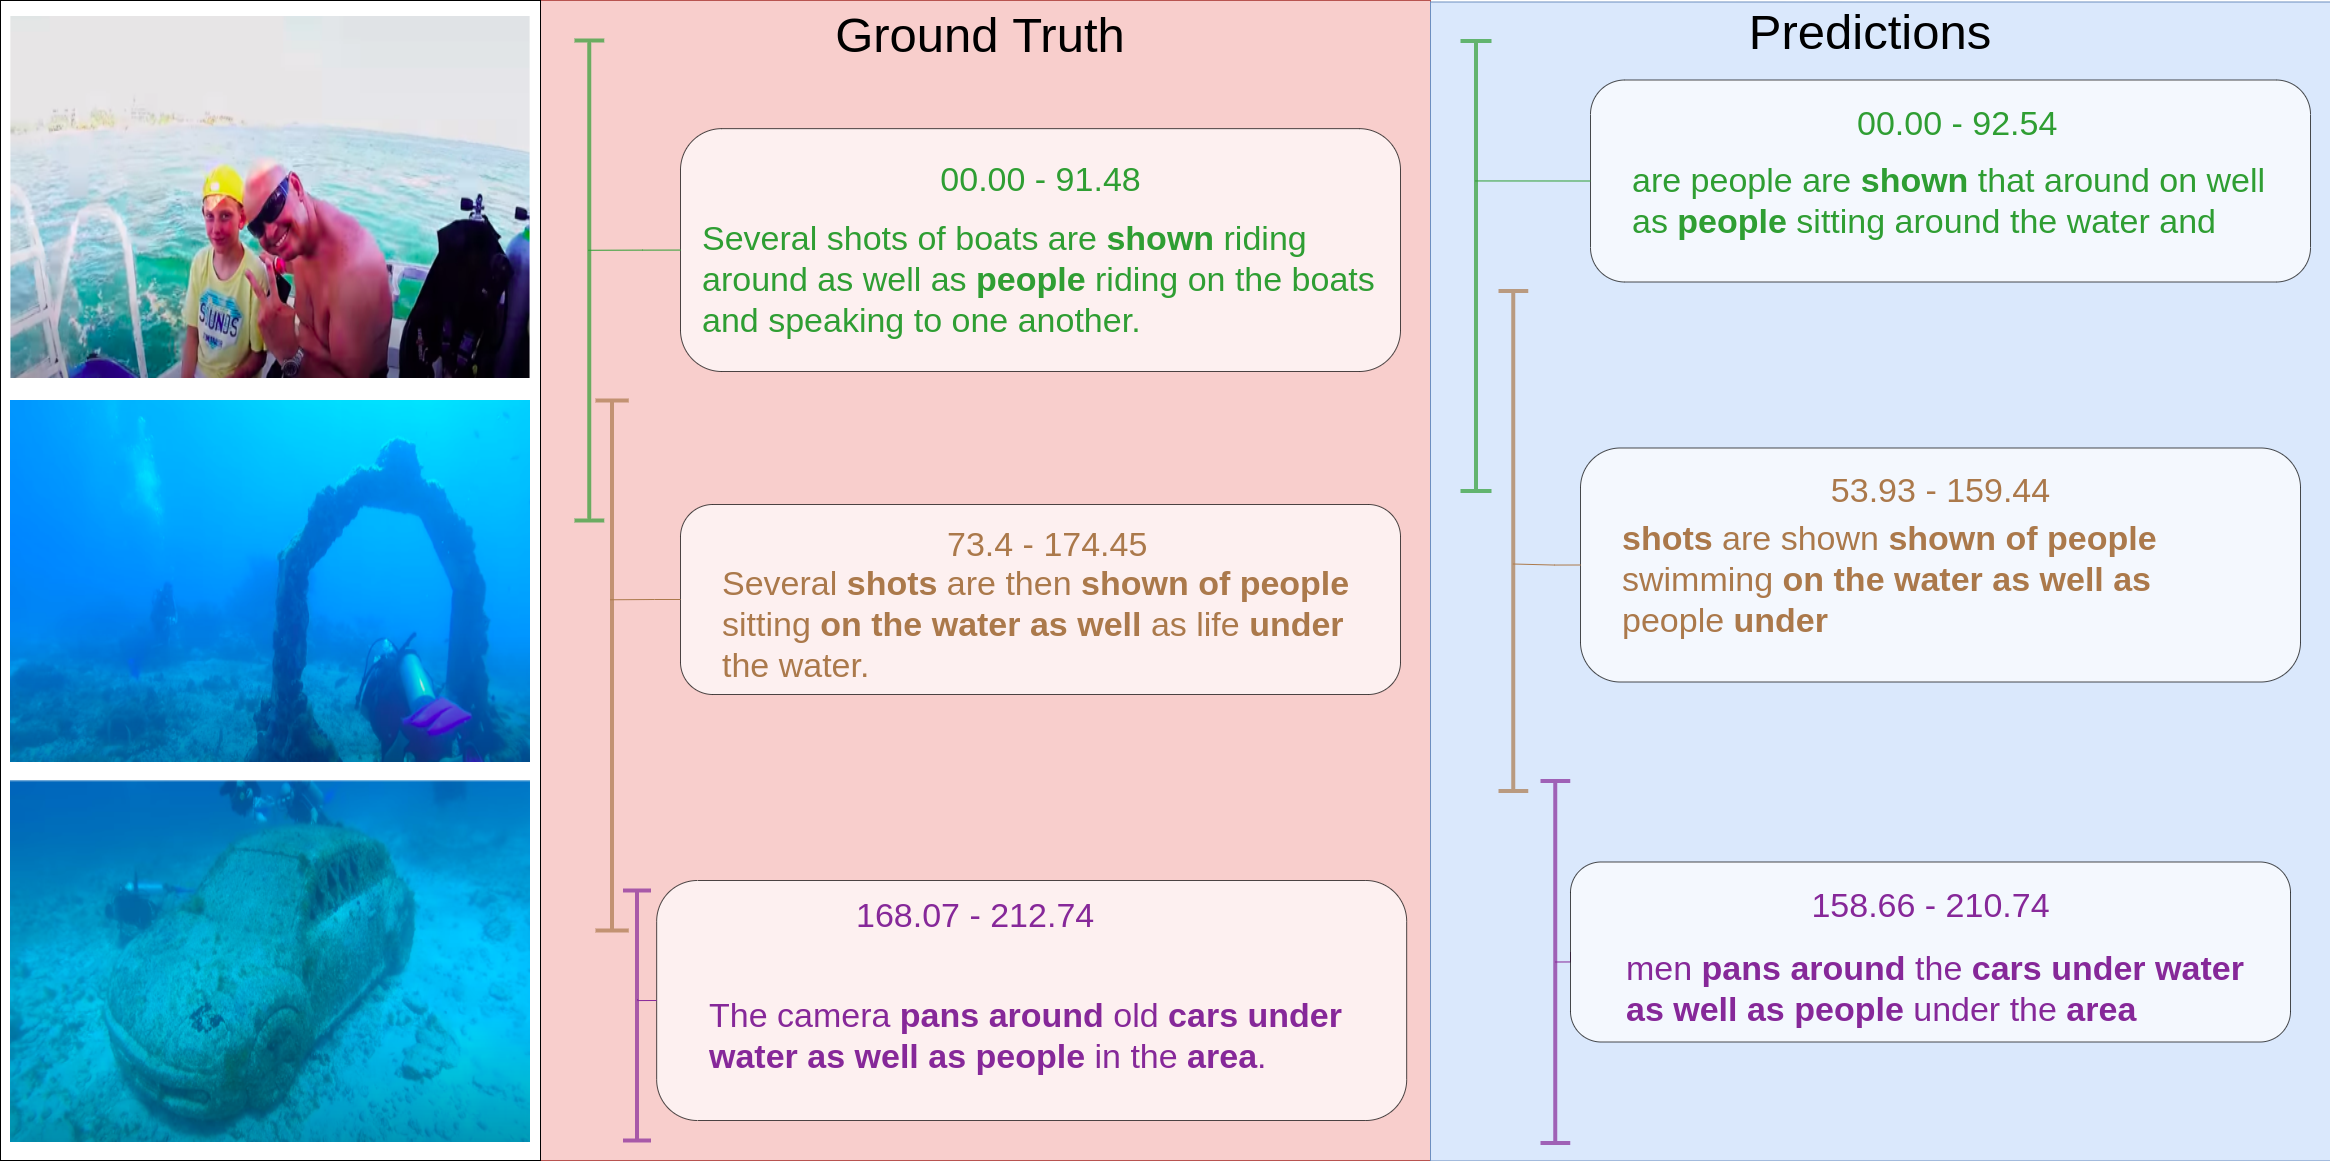
\includegraphics[width=\linewidth] {assets/img/dvc-segments/FsS_NCZEfaI.png}
    \end{subfigure}%
	\vspace{4mm}
    \begin{subfigure}[b]{\linewidth}
        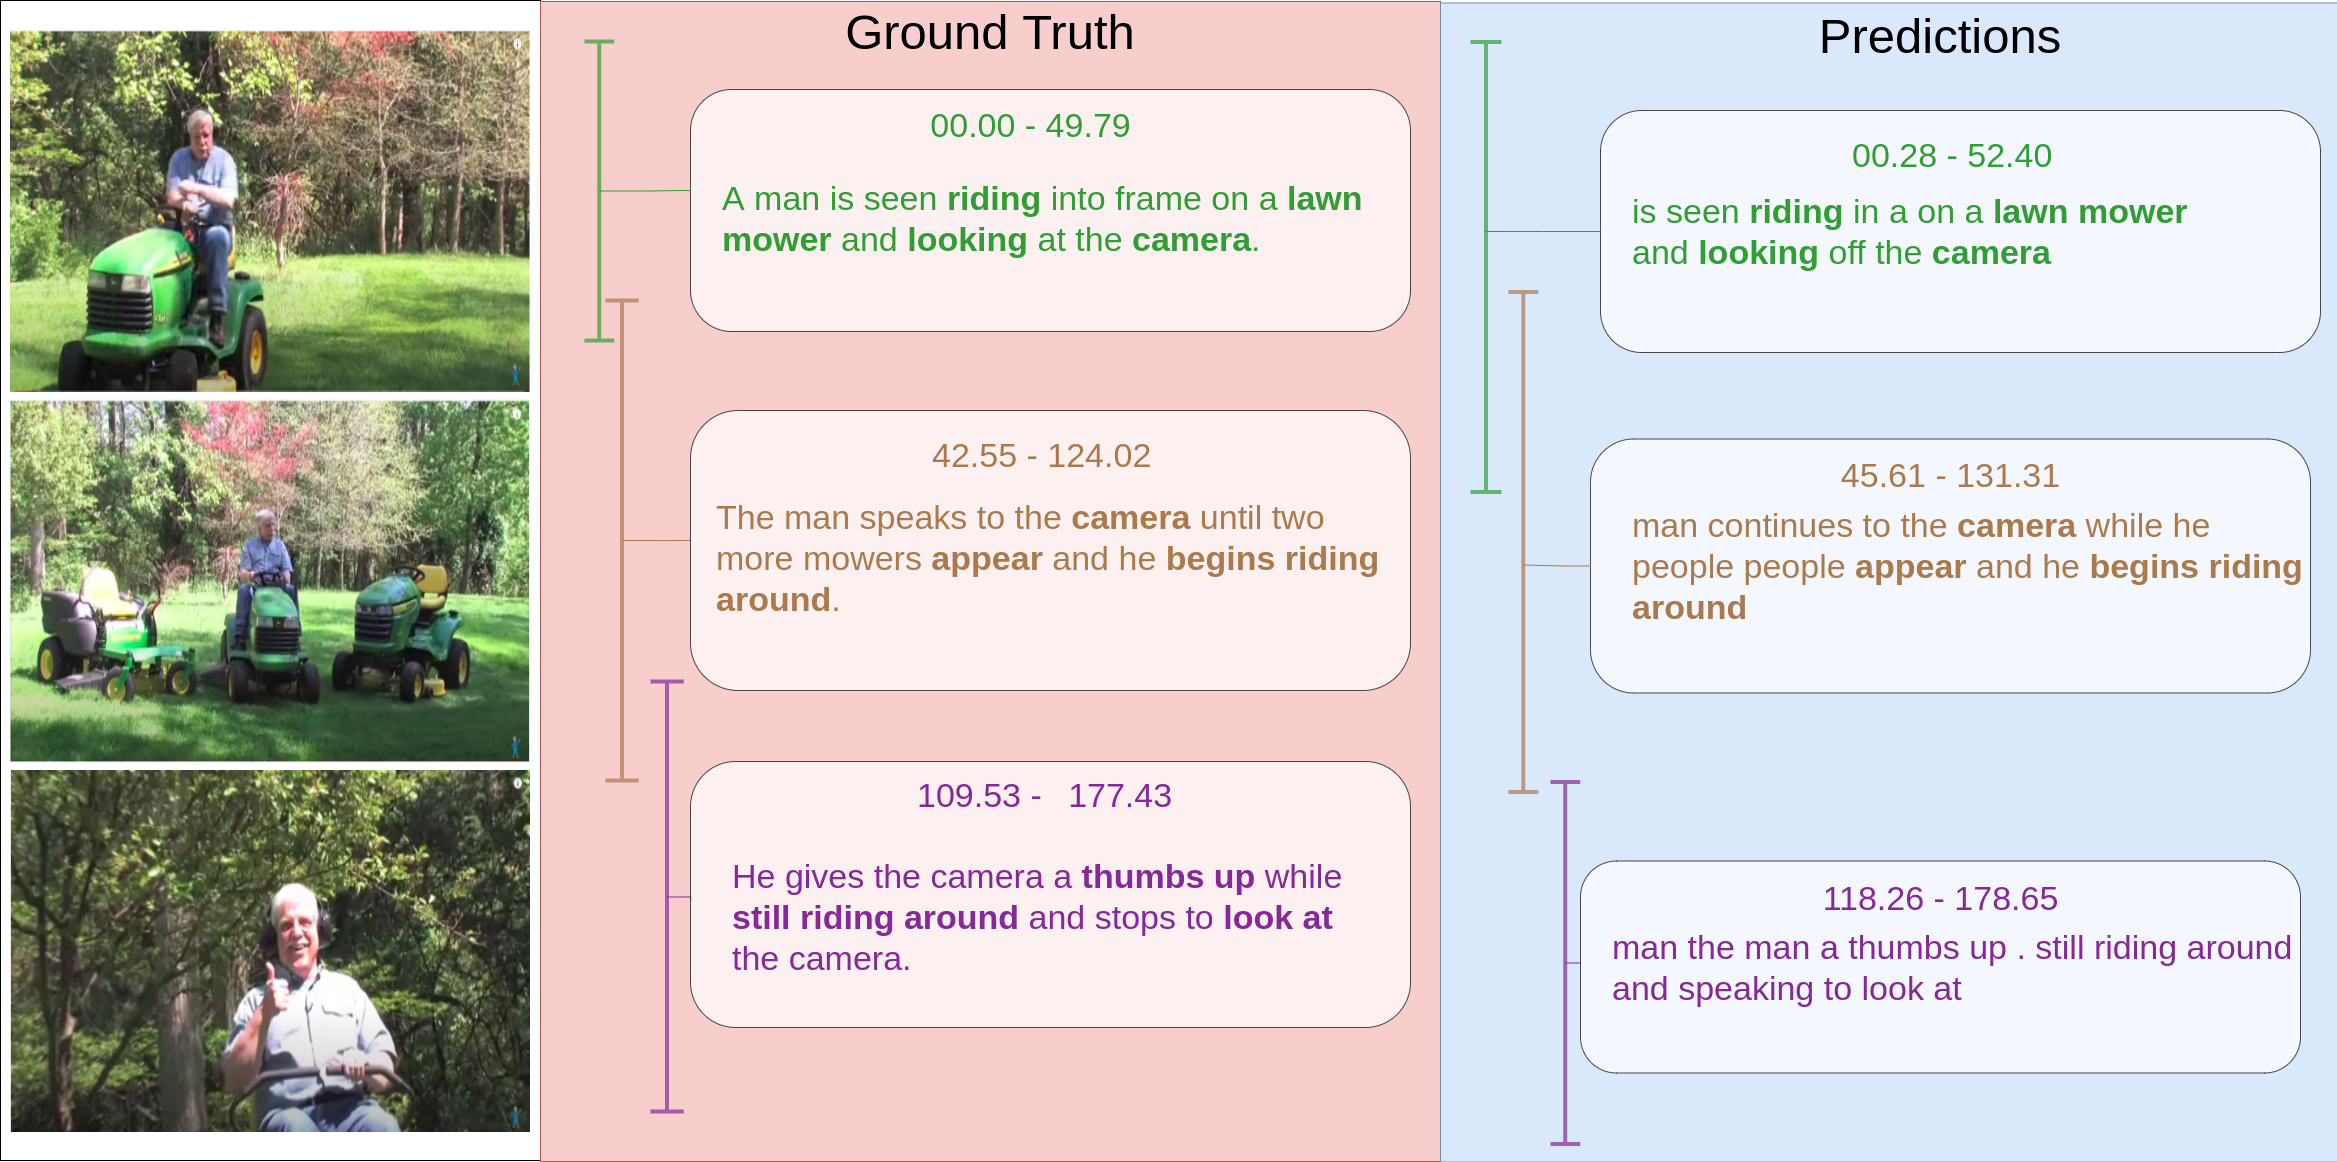
\includegraphics[width=\linewidth] {assets/img/dvc-segments/puK4NxGKNdQ.png}
    \end{subfigure}
    \caption{Visualization for predicted proposal segments and captions on ActivityNet Captions Dataset (validation set)}

	\label{fig:dvc-segments-1}
\end{figure}

\begin{figure}
	\centering
	\includegraphics[width=\linewidth] {assets/img/dvc-segments/qI1ZayfiGHI.png}
	\caption{Visualization for predicted proposal segments and captions on ActivityNet Captions Dataset (validation set)}
	\label{fig:dvc-segments-2}
\end{figure}


